\documentclass[11pt]{article}

\usepackage[a4paper,margin=1in]{geometry}
\usepackage{amsmath,amssymb}
\usepackage{siunitx}
\usepackage{graphicx}
\usepackage{hyperref}
\usepackage{caption}
\usepackage{subcaption}

\title{Seeing Inside:  The Radon Transform, MATLAB Experiments,\\
       and Biomedical Imaging Applications}
\author{autor\\
        PhD Student, Biomedical Engineering}
\date{\today}

\begin{document}
\maketitle

\begin{abstract}
The Radon transform links pure mathematics with life--saving medical
technology.  This report introduces the transform, demonstrates analytic
and numerical examples in MATLAB, and explains how filtered
back-projection underpins modern computed tomography (CT).
All experiments and figures were produced with a MATLAB Live Script;
figure file names are indicated for reproducibility.
\end{abstract}

\tableofcontents
\bigskip

%%%%%%%%%%%%%%%%%%%%%%%%%%%%%%%%%%%%%%%%%%%%%%%%%%%%%%%%%%%%%%%%%%%%%%%%
\section{Introduction}

Computed tomography (CT) revolutionised diagnostic radiology by allowing
physicians to reconstruct cross-sectional images of internal anatomy
from line–integral measurements of X-ray attenuation.
Mathematically, these line integrals form the \emph{Radon transform},
introduced by Johann Radon in 1917 \cite{Radon1917}.  
This report summarises the theory, reproduces textbook examples, and
documents hands-on MATLAB explorations relevant to biomedical
engineering practice.

%%%%%%%%%%%%%%%%%%%%%%%%%%%%%%%%%%%%%%%%%%%%%%%%%%%%%%%%%%%%%%%%%%%%%%%%
\section{Theory of the Radon Transform}

For a function \( f(x,y) \) on \( \mathbb R^{2} \),
its Radon transform \( \mathcal R f \) is the set of line
integrals
\begin{equation}
  \bigl(\mathcal R f\bigr)(p,\varphi)
  \;=\;
  \int_{-\infty}^{\infty}
    f\!\bigl(p\cos\varphi - s\sin\varphi,\;
             p\sin\varphi + s\cos\varphi\bigr)\; \mathrm ds,
  \label{eq:radon-def}
\end{equation}
where \( p \) is the signed distance of the line from the origin and
\( \varphi \) is the angle the line’s normal makes with the \(x\)-axis.
Recovering \(f\) from \( \mathcal R f \) is the \emph{inverse Radon
transform}.  The Fourier Slice Theorem shows that a 1-D inverse Fourier
transform of each projection, followed by a 2-D inverse transform,
re-creates \(f\).  Numerically this leads to
\emph{filtered back-projection} (FBP), implemented in MATLAB as
\texttt{iradon}.

%%%%%%%%%%%%%%%%%%%%%%%%%%%%%%%%%%%%%%%%%%%%%%%%%%%%%%%%%%%%%%%%%%%%%%%%
\section{Analytic Experiments}

\subsection{Radially symmetric Gaussian}

Using the Symbolic Math Toolbox we verified that a centred Gaussian
\[
  f(x,y)=\exp\!\bigl(-(x^{2}+y^{2})\bigr)
\]
has a Radon transform independent of \( \varphi \):
\(
  (\mathcal R f)(p,\varphi)=\sqrt{\pi}\,\exp(-p^{2})
\).
Figure~\ref{fig:gaussian} juxtaposes the surface plot of \(f\) and the
graph of its transform.

\begin{figure}[h]
\centering
\begin{subfigure}[b]{0.47\textwidth}
  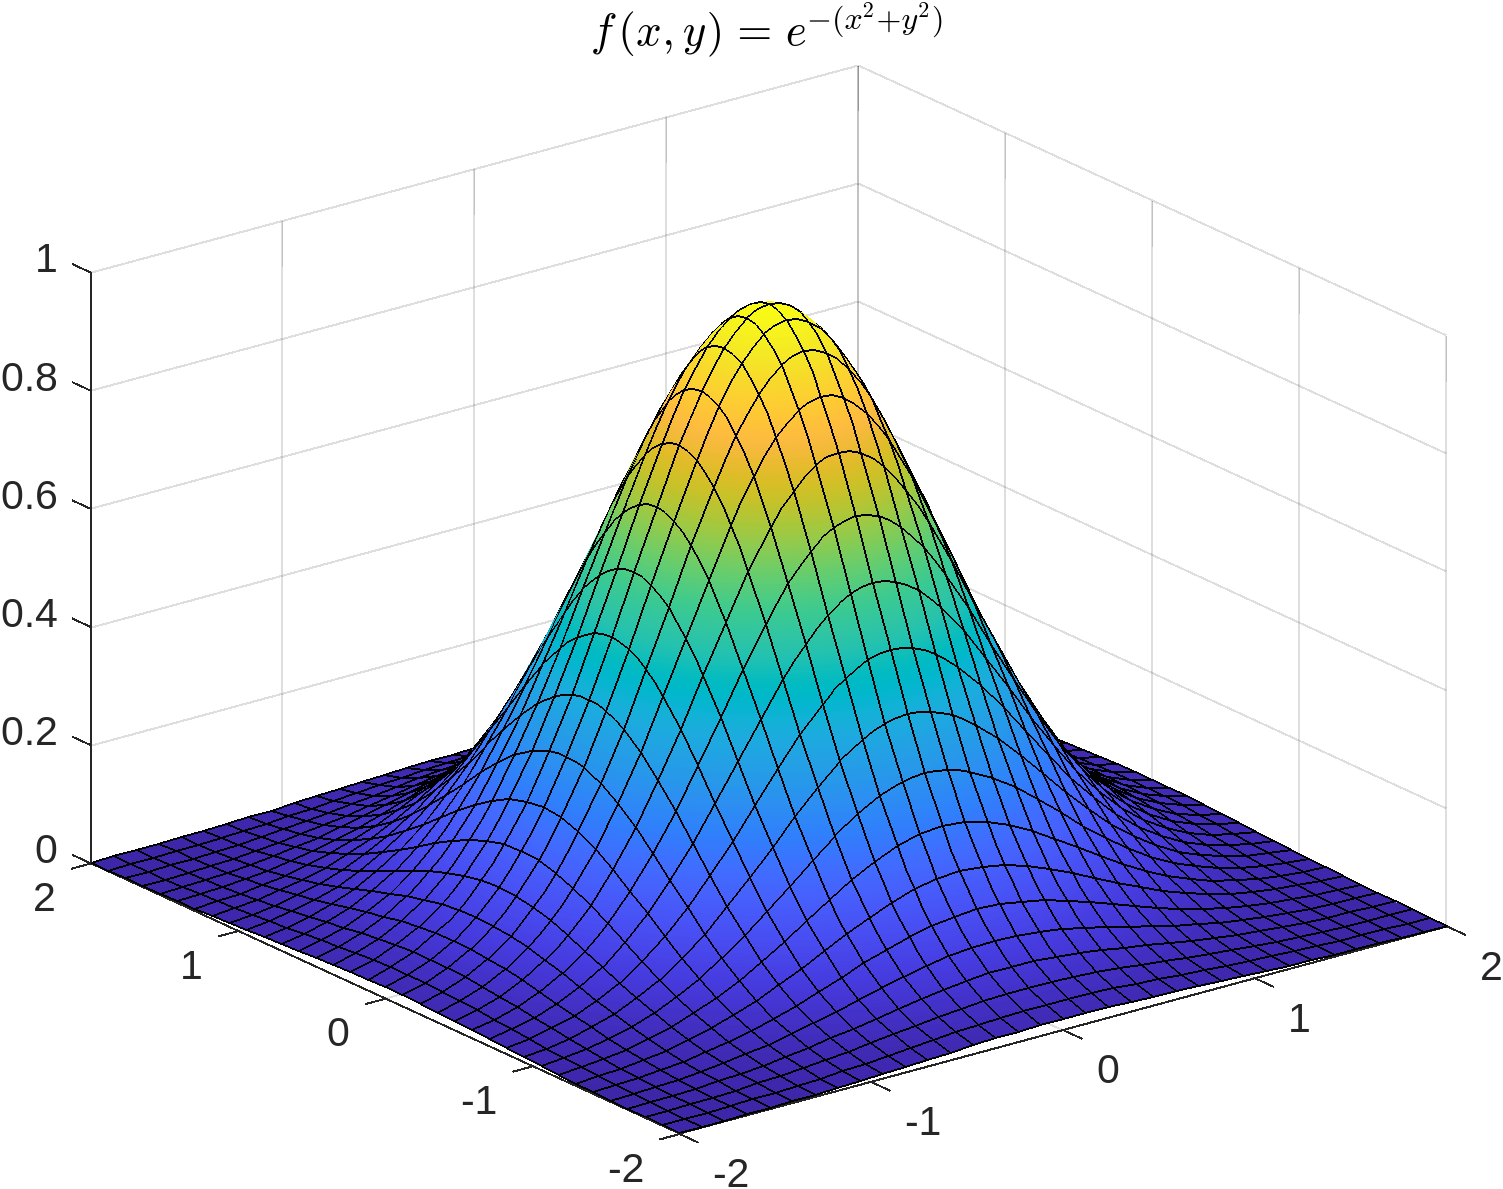
\includegraphics[width=\linewidth]{gaussian_surface.png}
  \caption{3-D surface of \(f\).}
\end{subfigure}
\hfill
\begin{subfigure}[b]{0.47\textwidth}
  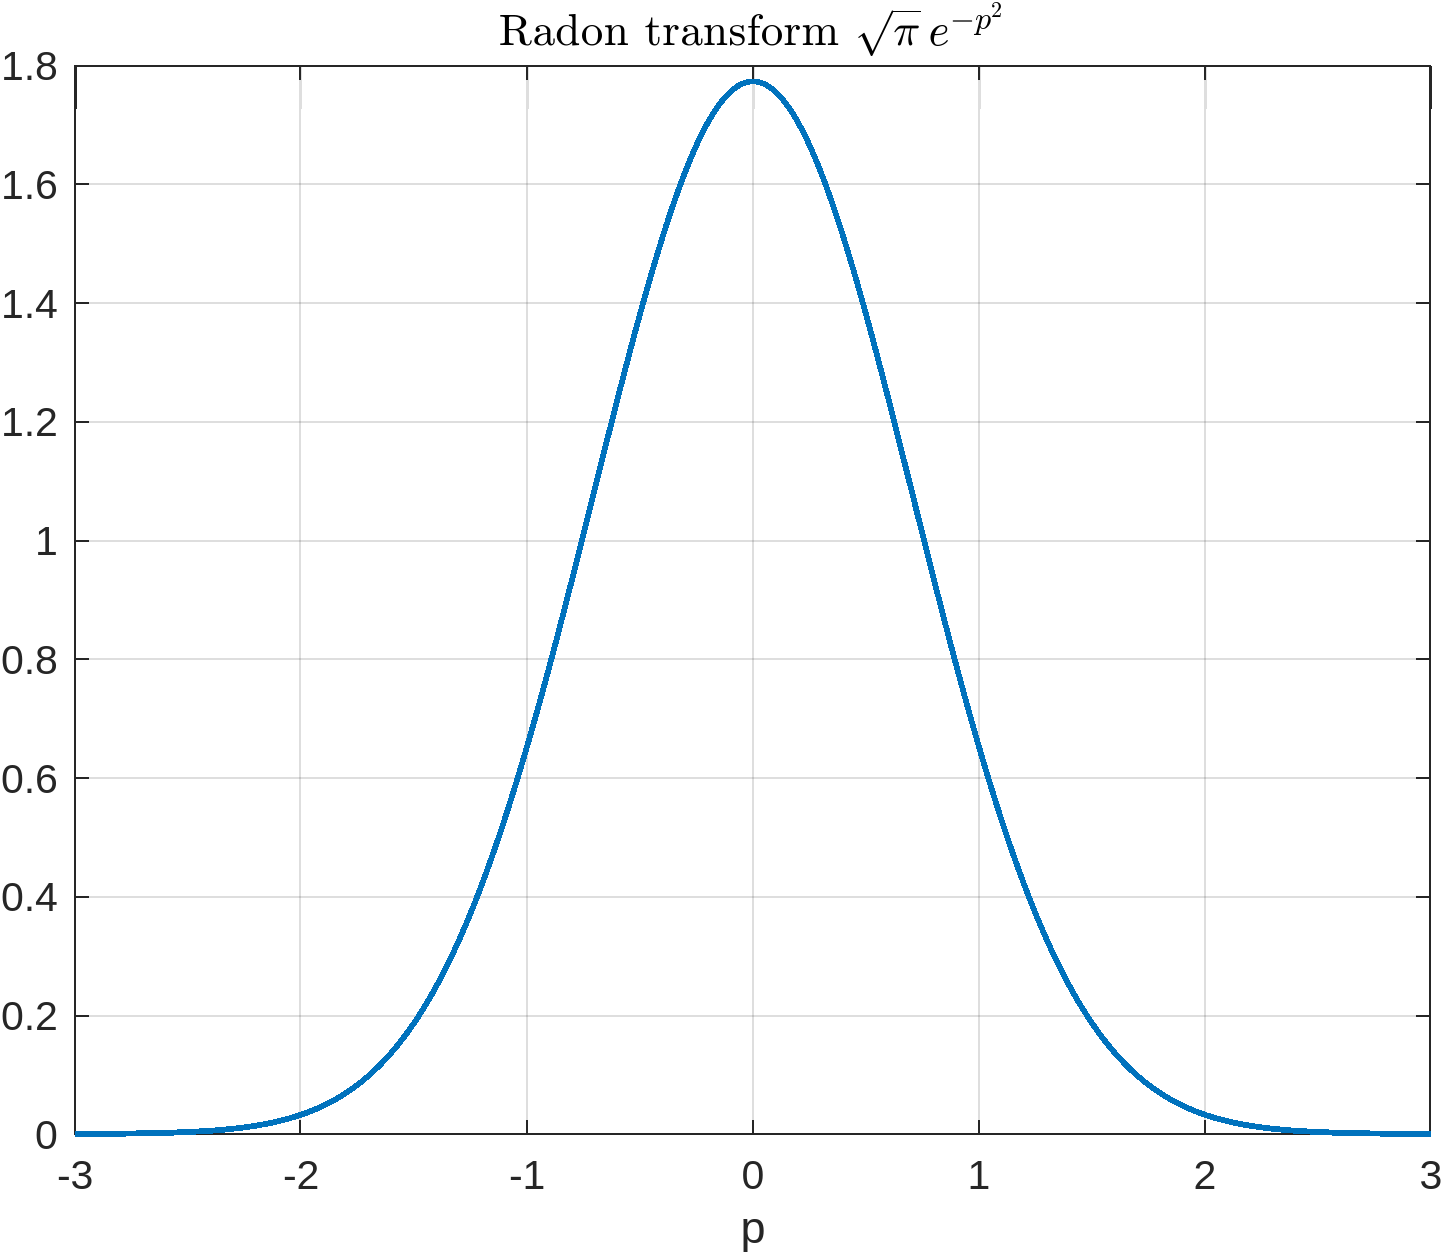
\includegraphics[width=\linewidth]{gaussian_radon.png}
  \caption{Radon transform vs.\ \(p\).}
\end{subfigure}
\caption{Radially symmetric example.}
\label{fig:gaussian}
\end{figure}

\subsection{Asymmetric polynomial–Gaussian}

Replacing the integrand by
\( g(x,y)=(x^{2}+3y^{2})e^{-(x^{2}+y^{2})} \)
breaks the circular symmetry; the resulting transform depends on
both \(p\) and \(\varphi\) (analytical expression omitted for brevity).
Figure~\ref{fig:asymmetric} shows density plots of \(g\) and
\(\mathcal Rg\).

\begin{figure}[h]
\centering
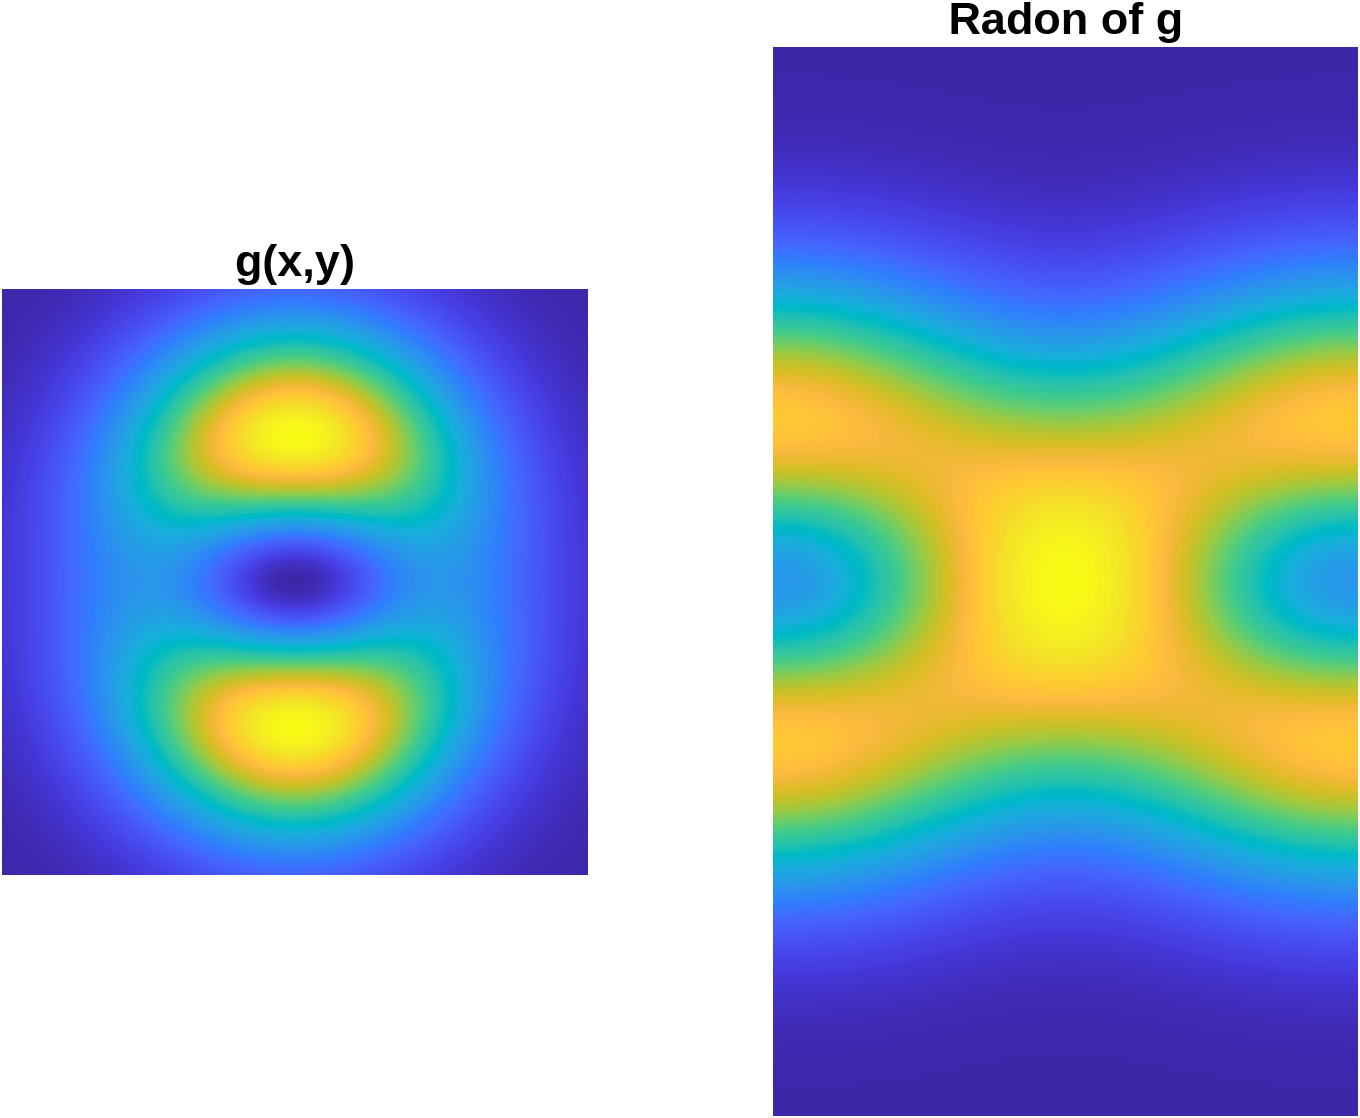
\includegraphics[width=\textwidth]{asymmetric_function_and_radon.png}
\caption{Density maps of the asymmetric test function (left) and its
Radon transform (right).\label{fig:asymmetric}}
\end{figure}

%%%%%%%%%%%%%%%%%%%%%%%%%%%%%%%%%%%%%%%%%%%%%%%%%%%%%%%%%%%%%%%%%%%%%%%%
\section{Discrete Radon Transform Experiments}

All remaining experiments use MATLAB’s discrete \texttt{radon} and
\texttt{iradon} functions.

\subsection{Binary disk phantom}

Figure~\ref{fig:disk} demonstrates how 180 projections of a simple disk
(representing, e.g.\ a cross-section of an organ) produce a
\emph{sinogram}, which FBP then reconstructs nearly perfectly.

\begin{figure}[h]
\centering
\begin{subfigure}[b]{0.30\textwidth}
  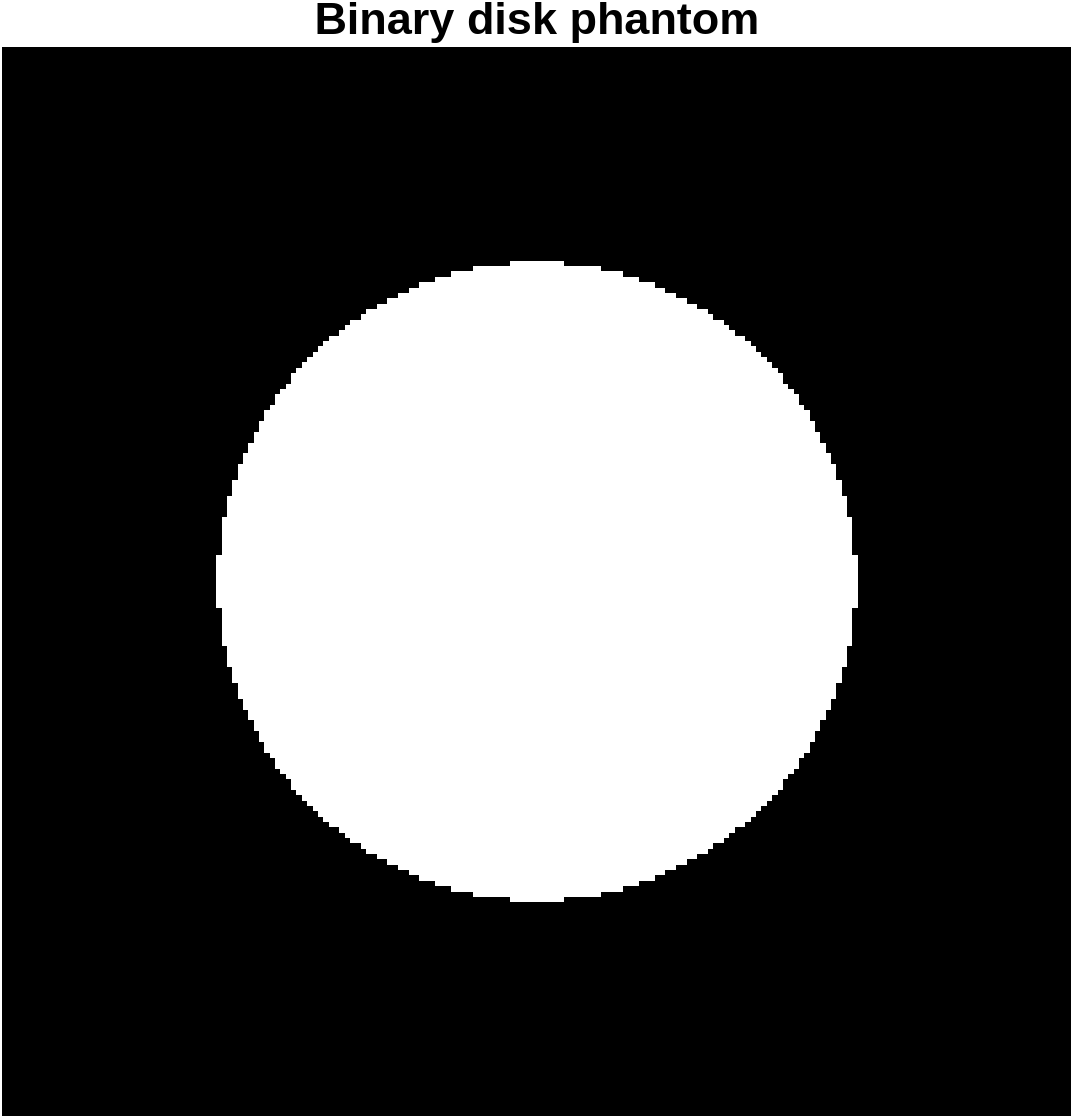
\includegraphics[width=\linewidth]{disk_original.png}
  \caption{Original image.}
\end{subfigure}
\hfill
\begin{subfigure}[b]{0.34\textwidth}
  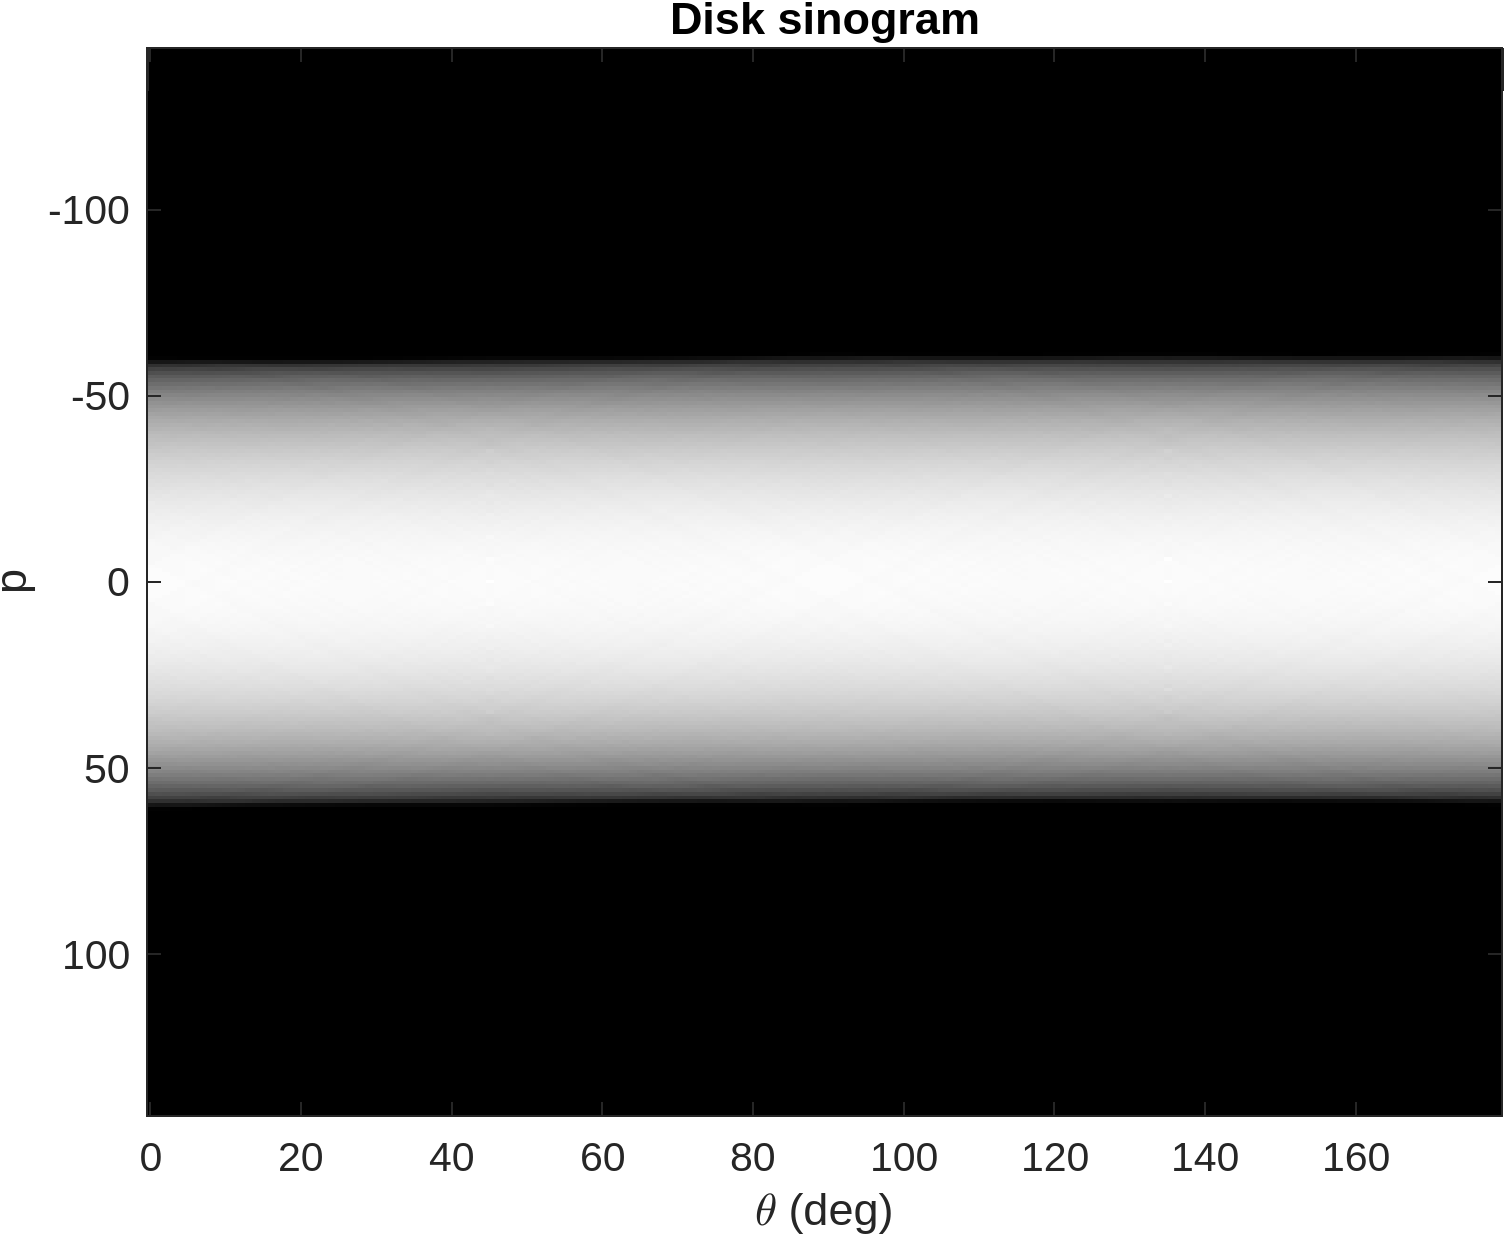
\includegraphics[width=\linewidth]{disk_sinogram.png}
  \caption{Sinogram.}
\end{subfigure}
\hfill
\begin{subfigure}[b]{0.30\textwidth}
  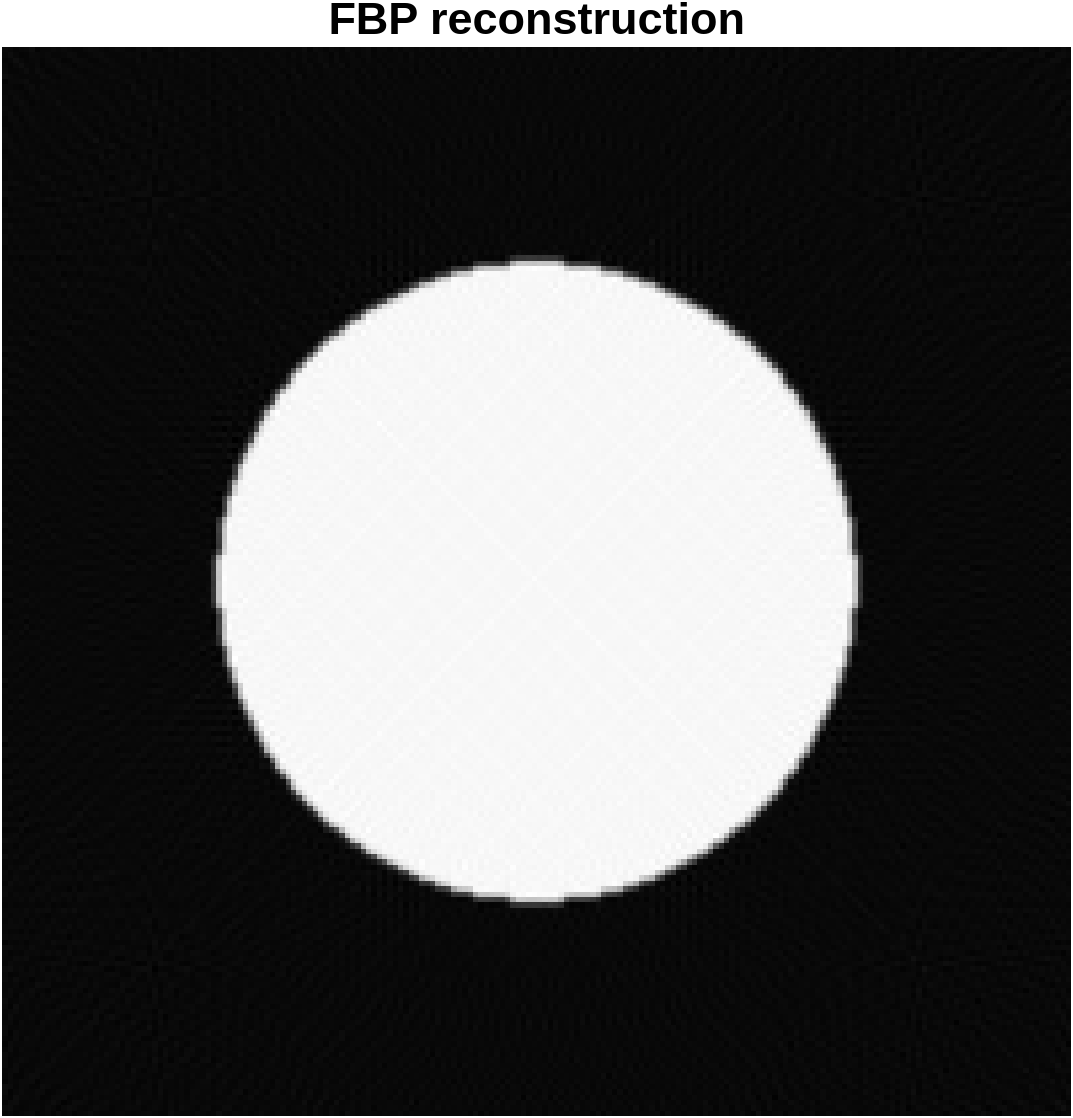
\includegraphics[width=\linewidth]{disk_reconstruction.png}
  \caption{FBP reconstruction.}
\end{subfigure}
\caption{Parallel-beam CT simulation of a disk phantom.}
\label{fig:disk}
\end{figure}

\subsection{Shepp–Logan head phantom}

The Shepp–Logan phantom is a synthetic yet realistic CT head slice.
With $180$ projections we obtain the results in
Figure~\ref{fig:phantom}.  
Qualitatively the reconstruction captures fine structures such as the
ventricles, illustrating clinical usefulness.

\begin{figure}[h]
\centering
\begin{subfigure}[b]{0.30\textwidth}
  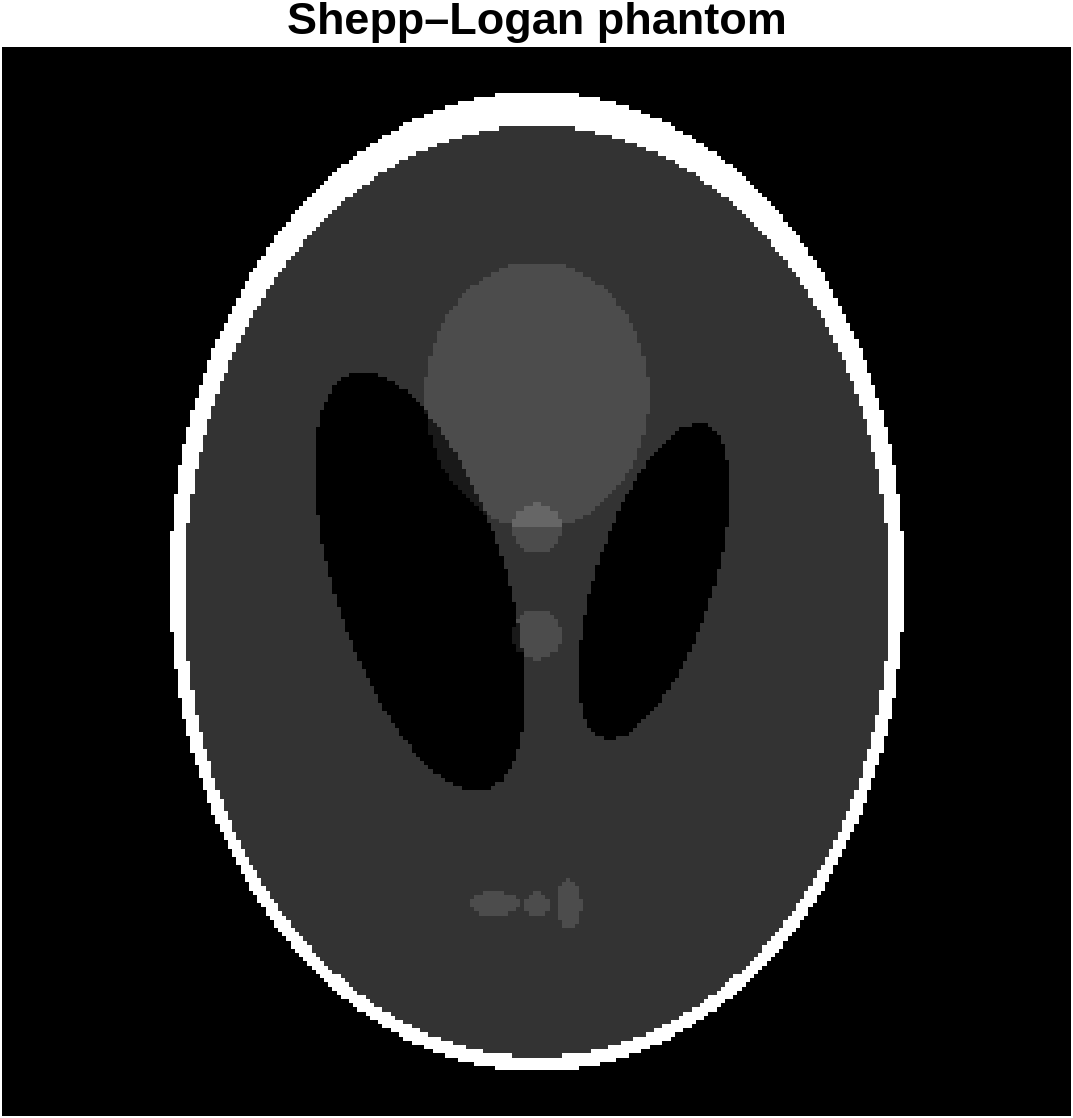
\includegraphics[width=\linewidth]{phantom_original.png}
  \caption{Ground truth.}
\end{subfigure}
\hfill
\begin{subfigure}[b]{0.34\textwidth}
  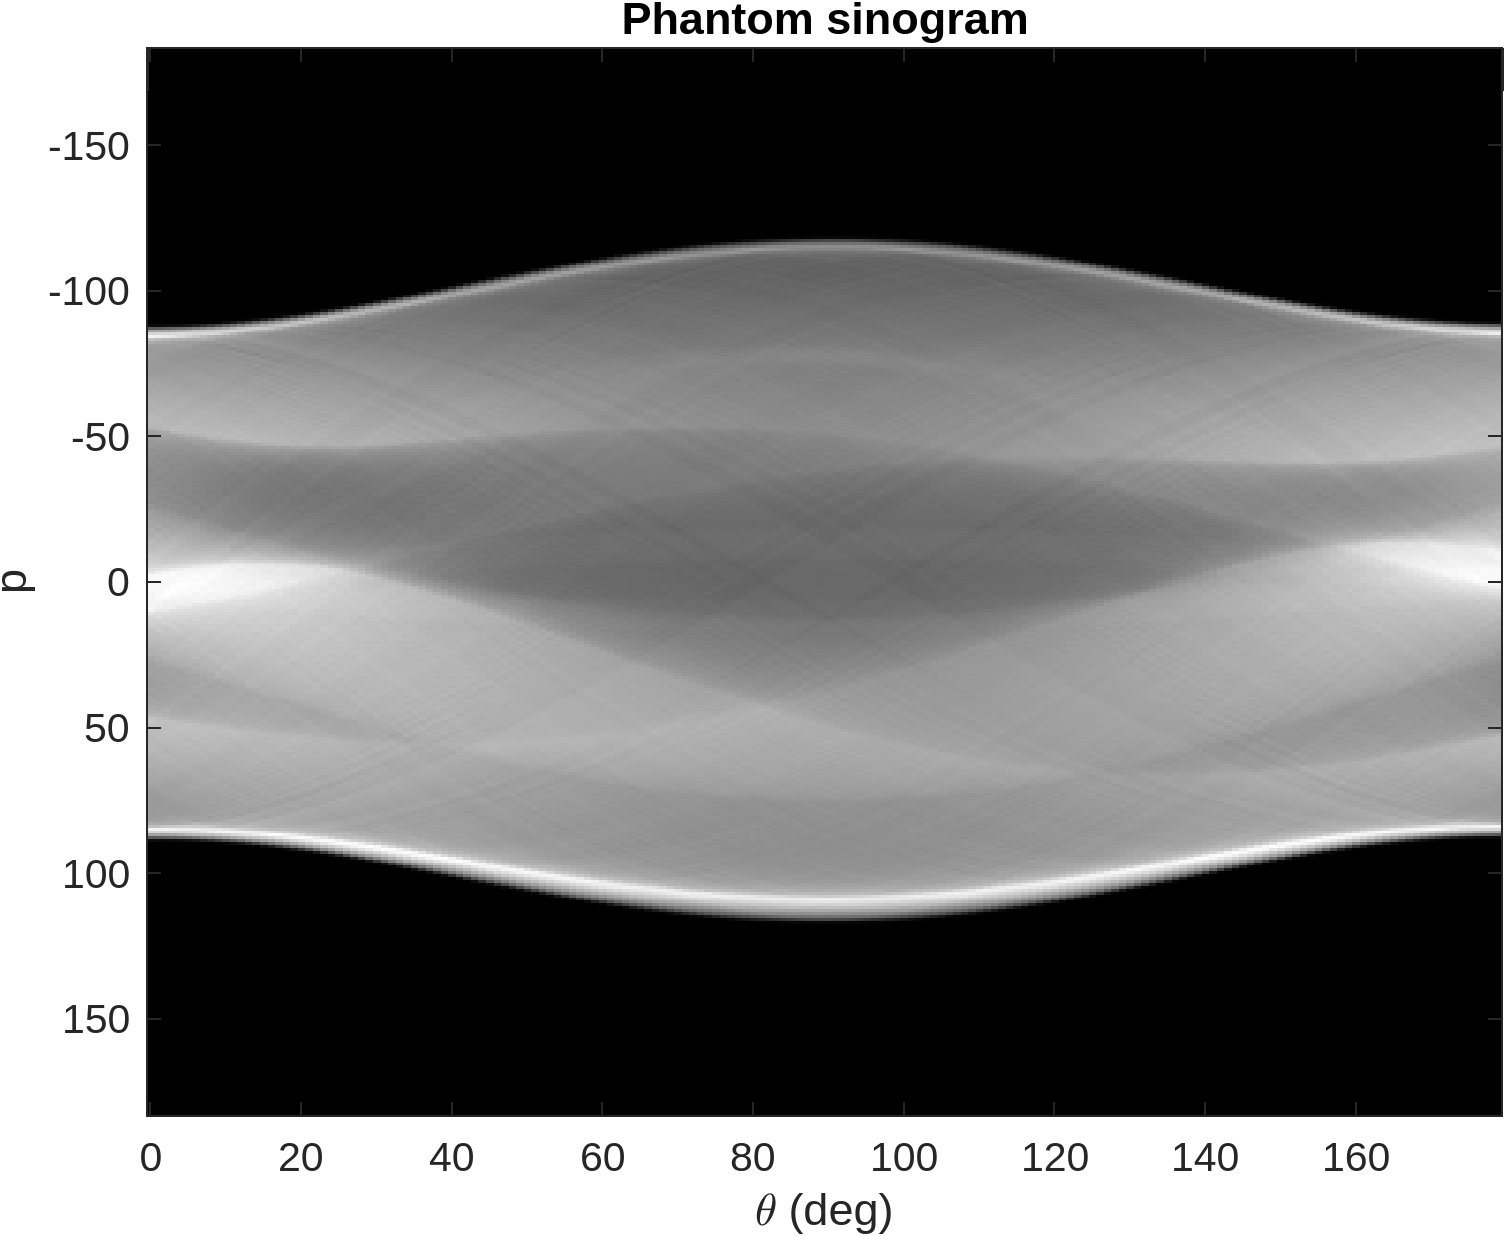
\includegraphics[width=\linewidth]{phantom_sinogram.png}
  \caption{Sinogram.}
\end{subfigure}
\hfill
\begin{subfigure}[b]{0.30\textwidth}
  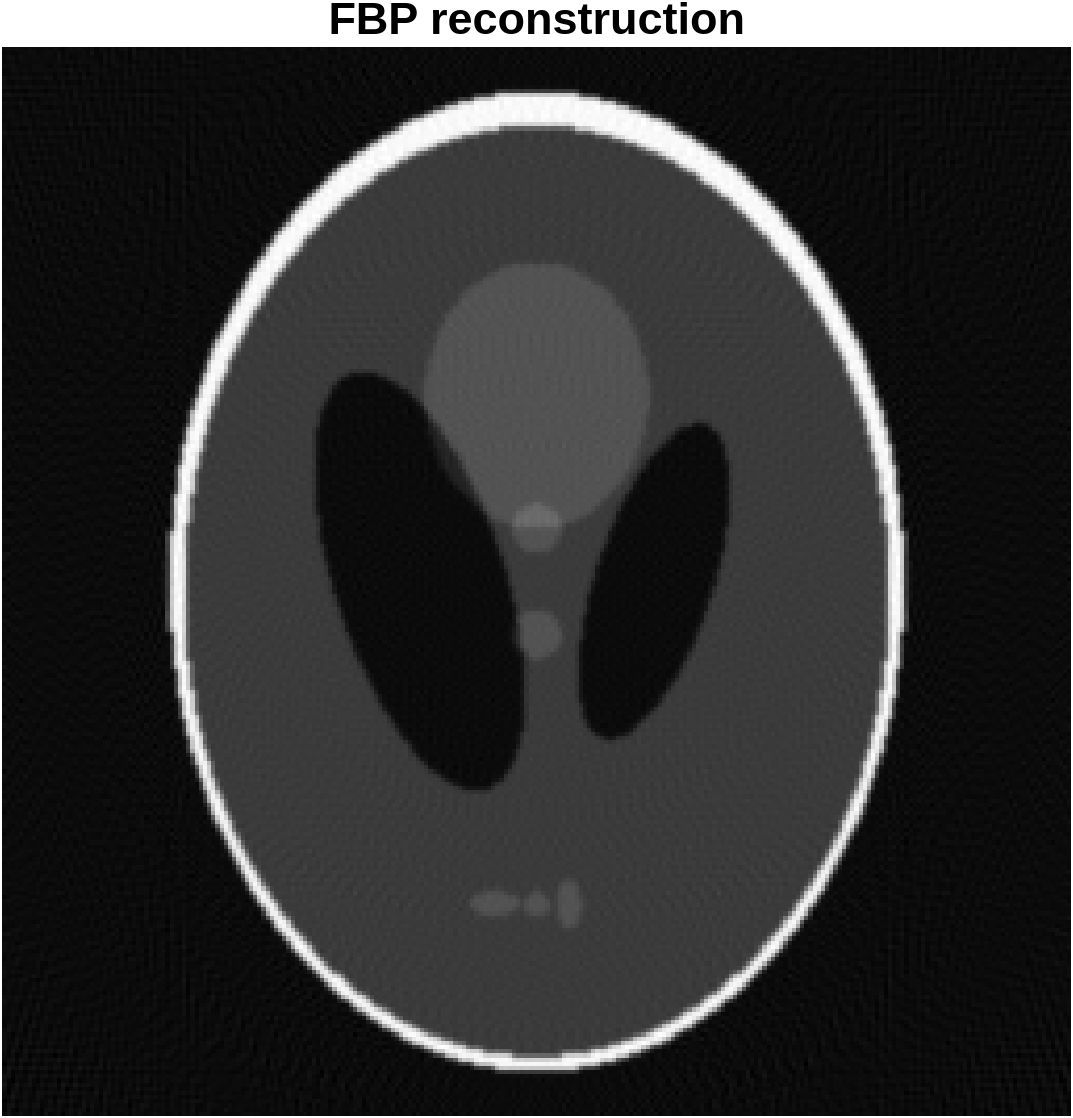
\includegraphics[width=\linewidth]{phantom_reconstruction.png}
  \caption{Reconstruction.}
\end{subfigure}
\caption{Shepp–Logan head phantom experiment.}
\label{fig:phantom}
\end{figure}

%%%%%%%%%%%%%%%%%%%%%%%%%%%%%%%%%%%%%%%%%%%%%%%%%%%%%%%%%%%%%%%%%%%%%%%%
\section{Biomedical Imaging Context}

\subsection{From mathematics to CT scanners}

In practice, modern scanners collect fan- or cone-beam projections while
rotating around the patient.  Proprietary reconstruction pipelines apply
noise correction, calibration, and iterative or FBP algorithms.
Nevertheless, Equation~\eqref{eq:radon-def} and its inversion remain the
core.  Figure~\ref{fig:mri} uses MATLAB’s built-in \texttt{mri} volume
to visualise slices akin to clinical data.

\begin{figure}[h]
\centering
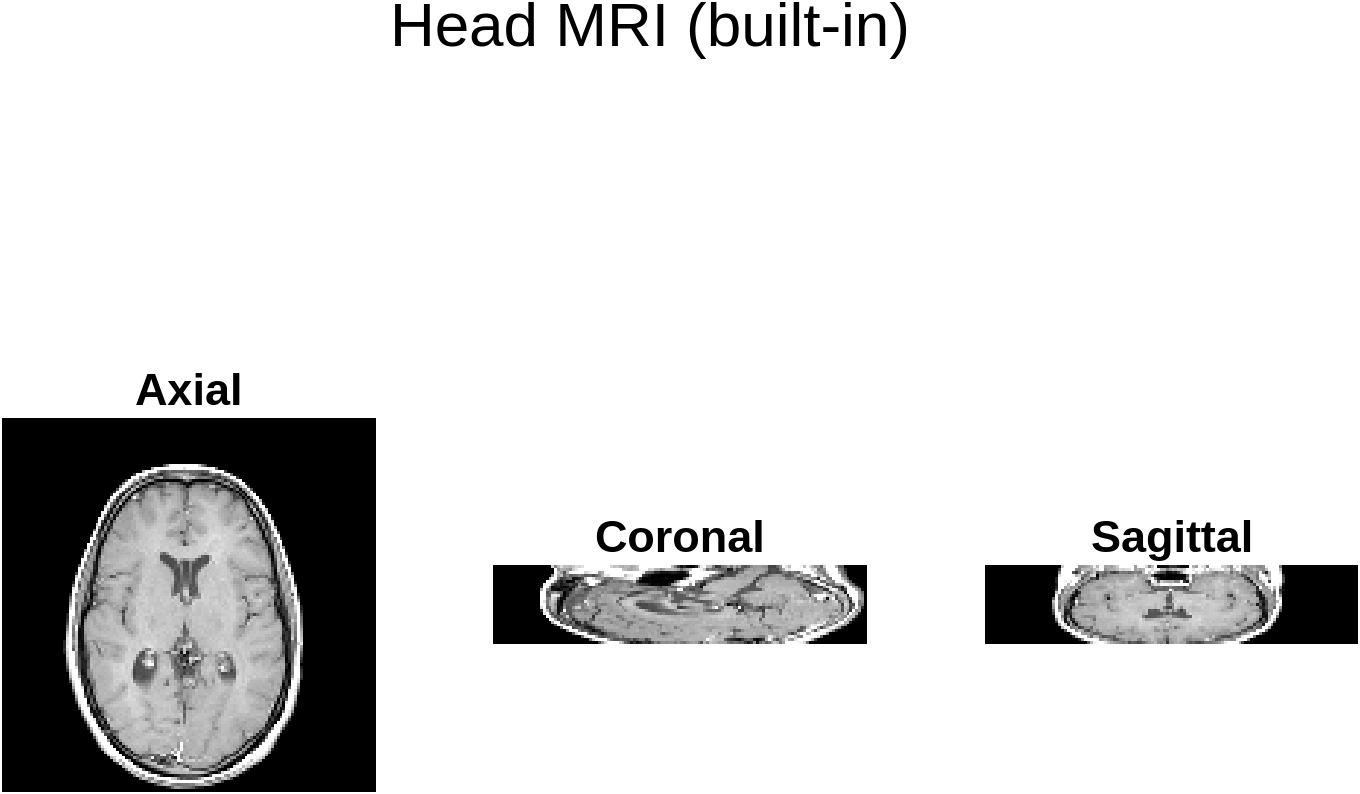
\includegraphics[width=0.6\textwidth]{mri_volume.png}
\caption{Orthogonal slices of MATLAB’s demo MRI data.  Each axial slice
can be reconstructed individually via the inverse Radon transform when
acquired in projection space.\label{fig:mri}}
\end{figure}

\subsection{Impact and future directions}

Beyond CT, Radon-type transforms appear in:
\begin{itemize}\itemsep0.2em
\item \textbf{Positron Emission Tomography (PET)}---employing coincident
      $\gamma$-ray detection.
\item \textbf{Optical projection tomography} for mesoscopic specimens.
\item \textbf{Electron microscopy} tilt-series reconstruction.
\item \textbf{Barcode decoding} (1-D Radon in scanners).
\end{itemize}

Emerging research combines deep learning with classical FBP to reduce
radiation dose while preserving diagnostic quality.

%%%%%%%%%%%%%%%%%%%%%%%%%%%%%%%%%%%%%%%%%%%%%%%%%%%%%%%%%%%%%%%%%%%%%%%%
\section{Conclusion}

Through analytic proofs and MATLAB simulations I gained intuition for
how line integrals over an object encode its structure, and how inverse
methods---especially filtered back-projection---turn those measurements
into images that guide clinical decisions.  The Radon transform thus
beautifully exemplifies the synergy between mathematics, computation,
and biomedical engineering.

%%%%%%%%%%%%%%%%%%%%%%%%%%%%%%%%%%%%%%%%%%%%%%%%%%%%%%%%%%%%%%%%%%%%%%%%
\begin{thebibliography}{9}
\bibitem{Radon1917}
J.~Radon, \emph{Über die Bestimmung von Funktionen durch ihre Integralwerte
längs gewisser Mannigfaltigkeiten}, Ber.\ Sächs.\ Akad.\ Wiss.\ Leipzig,
Math.-Phys.\ Kl.\ \textbf{69} (1917), 262–277.

\bibitem{CormackHounsfield}
A.~Cormack and G.~N.~Hounsfield, \emph{Nobel Lectures in Physiology or Medicine
1979}, Nobel Foundation, Stockholm, 1980.

\end{thebibliography}

\end{document}
